\documentclass[12pt,a4paper,oneside]{book} 
\usepackage[utf8]{inputenc}
\usepackage[spanish]{babel}
\usepackage{amsmath}
\usepackage{amsfonts}
\usepackage{amssymb}
\usepackage{abstract} % Allows abstract customization
\renewcommand{\abstractnamefont}{\normalfont\bfseries} % Set the "Abstract" text to bold
\renewcommand{\abstracttextfont}{\normalfont\small\itshape} % Set the abstract itself to small italic text


\usepackage{amssymb, amsmath}
\usepackage{graphicx}
\usepackage[left=2.54cm,right=2.54cm,top=2.54cm,bottom=2.54cm]{geometry}

\begin{document}
	
	\thispagestyle{empty} 
	
	\begin{center} 
		\LARGE{UNIVERSIDAD PRIVADA DE TACNA} \\[0.5cm] 
		\Large{FACULTAD DE INGENIERÍA DE SISTEMAS}\\[0.5cm] 
		\large{ ESCUELA PROFESIONAL DE INGENIERÍA SISTEMAS} 
	\end{center}
	
	\begin{figure}[htb]
		\centering 
\includegraphics[width=6cm, height=7cm]{img/uptlogo.jpg}
	\end{figure}
	
	\begin{center} 
			\LARGE{\bf PROYECTO TRABAJO FINAL \newline UNIDAD I }\\ \vspace{.25cm}
		
	\end{center}

	\begin{center} 
		
		\textbf {CURSO}\\ 
		\large Base de Datos II \\
		
		\textbf {DOCENTE}\\
		\large Mag. Patrick Cuadros Quiroga\\
	
		\textbf {INTEGRANTES}\\
		\large Tarqui Montalico, Risther Jaime - 2017057469 \\
		\large Limache Victorio, V\'ictor Piero - 2017057857 \\
		\large Callata Flores, Mart\'in Rafael - 2015053847 \\
		\large S\'anchez Rodr\'iguez, Bayron - 2017057859 \\
		\large Liendo Velasquez, Joaqu\'in - 2016054463 \\
		
		
	\end{center}

	
	
	\begin{center} 
		\Large \textsc{Tacna - Perú} \\
		\Large \textsc{2020 } 
	\end{center}

	\newpage
	
	%%INICIO abstract
	\begin{abstract}

		Un sistema de software de Escritorio basado en gestionar datos
		importantes de la empresa en las cuales podr\'a registrar el cliente y derivadamente a su mascota con la aplicaci\'on por parte del cliente, y por medio de la empresa podrá ver sus clientes, el registro de empleados, las ventas de medicamentos en las cuales se realizar\'a de una forma concisa y clara a las necesidades de la empresa, y así la veterinaria podrá obtener un espacio de registro m\'as sencillo y eficaz.\\
		
		El software est\'a basado en escritorio como antes mencionado, en un lenguaje de aplicaci\'on llamada “(C Sharp)” con la finalidad de adaptarse al sistema operativo Windows desde W7 hacia adelante, la aplicación está plenamente desarrollado para el uso dentro de la Empresa, mas no de los clientes. A su vez al desarrollar este programa puede ser que haya determinadas fallas del software en las cuales utilizaremos la aplicación SonarQube para el mejoramiento de dicha aplicación. \\
		\begin{center}
			
			\textbf{Abstract}
		\end{center}
		A Desktop software system based on managing data
		important of the company in which you can register the client and, consequently, your pet with the application by the client, and through the company you can see its clients, the registration of employees, the sales of medicines in which the a concise and clear way to the needs of the company, and thus the veterinarian can obtain a simpler and more efficient registration space.\\
		
		The software is based on the desktop as mentioned before, in an application language called "(C Sharp)" in order to adapt to the Windows operating system from W7 onwards, the application is fully developed for use within the Company, more not from customers. In turn, when developing this program, it may be that there are certain software flaws in which we will use the SonarQube application to improve said application. \\
	\end{abstract}
	%%FIN abstract
	
	\newpage
	
	\begin{center} 
		\LARGE{\bf PROYECTO TRABAJO FINAL \newline UNIDAD I }\\ \vspace{.25cm}
	\end{center}

	
	\begin{enumerate}
		
		\item \textbf{Introducci\'on.} \\
		
				Una gran cantidad de empresas de nuestra región interactúan de forma directa con los clientes, no cuentan con un registro organizado ni automatizado, lo cual representa lentitud al momento de registrar algún pago o desbalance al momento de sacar las cuentas del d\'ia. \\
				
				La investigaci\'on planteada en este trabajo est\'a relacionada con el proceso de veterinaria Pet’s Planet ubicada Gral. Varela 233, Tacna, para el desarrollo del sistema de veterinaria se tuvo que usar las herramientas y los instrumentos necesario para la obtención de información tales como la encuesta realizada al dueño de la empresa para así poder identificar los procesos de funcionamiento de la veterinaria Pet’s Planet.\\
		
		
		\item \textbf{T\'itulo.}
		
				Sistema de Veterinaria “PET’S PLANET”.	
				
		\item \textbf{Autores.}
		
				\begin{itemize}
					
					\item	Limache Victorio, V\'ictor Piero 
					\item	Tarqui Montalico, Risther Jaime 
					\item	S\'anchez Rodr\'iguez, Bayron 
					\item	Liendo Velasquez, Joaqu\'in 
					\item	Callata Flores, Rafael 
					
				\end{itemize}
			
		\item \textbf{Planteamiento del problema.}
				\begin{enumerate}
					\item \textbf{Problema.} \\
					
					El problema de todo estudiante del cual empieza con el desarrollo de software de una manera principiante, es el no uso de m\'etricas que pueden ayudar a la calidad del c\'odigo al cual nosotros queremos implementar, es por eso que el programa actual del cual ya está desarrollado no cuenta con un uso correcto de m\'etricas, por lo tanto, este c\'odigo siempre puede optar por mejorar. \\
					
					La actualizaci\'on de este c\'odigo no debe afectar al funcionamiento del programa, pero s\'i a su rendimiento. Dicho esto, el código fuente actual puede ser mejorable.\\
					
					
					\item \textbf{Justificaci\'on.}
					
					Con el fin de mejorar la calidad del software” Veterinaria PET’S PLANET”, estos serían nuestros planteamientos que nos haremos:
					
					\begin{enumerate}
						
						\item \textbf{¿Qu\'e es lo que vamos de hacer?} \\
						
						 Una mejora al c\'odigo fuente del sistema Veterinaria PET’S PLANET con la herramienta SonarQube.\\
						
						\item \textbf{¿Por qu\'e se va hacer?} \\
						
						Para lograr la mejora del c\'odigo actual, sin modificar el proyecto.\\
						
						\item \textbf{¿Para qu\'e se va hacer?} \\
						 
						Para tener un mejor rendimiento del programa, y utilizar la herramienta que aprendimos a lo largo de la unidad: SonarQube.\\
						
						\item \textbf{¿C\'omo se va hacer?} \\ 
						
						Utilizando la herramienta SonarQube, y en la cual utilizaremos nuestros conocimientos aprendidos en el transcurso del curso para la mejora del software.\\
						
						\item \textbf{¿Por qu\'e es importante este trabajo de unidad?}\\
						
						Porque mejora el actual c\'odigo fuente y como consecuencia aumenta el rendimiento del sistema. \\
						
					\end{enumerate}
					
					\item \textbf{Alcance.}
					
						\begin{itemize}
							\item El Sistema contará con una base de datos ,en la nube.
							\item El Sistema contará de un control de Registros.
							\item Contará con reportes de Servicios.
							
						\end{itemize}
				\end{enumerate}
		\item \textbf{Referentes te\'oricos. } 
		
		\item \textbf{Objetivos. } 
				\begin{enumerate}
					\item \textbf{General.} \\
						Dise\~nar e implementar un software para mejorar de interacci\'on entre los clientes y la cl\'inica veterinaria.	
						
					\item \textbf{Espec\'ificos.}
					
					\begin{enumerate}
						
						\item Generar una base de datos que maneje informaci\'on de clientes, mascotas, productos y servicios para generar un an\'alisis hist\'orico.
						\item Proveer una interfaz pr\'actica y amigable para facilitar el uso de la plataforma a usuarios y m\'edicos veterinarios.
						\item Mostrar productos y servicios que ofrece la cl\'inica.
						\item Generar reportes de atenciones de cada m\'edico veterinario, as\'i como de los clientes y mascotas.
						
					\end{enumerate}
					
				\end{enumerate}
		\item \textbf{Referentes te\'oricos.}
			 \begin{enumerate}
			  	\item Un componente de software debe diseñarse e implementarse de modo que pueda volverse a usar en muchos programas diferentes. Los modernos componentes reutilizables incorporan tanto los datos como el procesamiento que se les aplica, lo que permite que el ingeniero de software cree nuevas aplicaciones a partir de partes susceptibles de volverse a usar [1].\\
			  	
			  	\item El mejoramiento del proceso de Software abarca un conjunto de actividades que conducirán a un mejor proceso de software y, en consecuencia, a software de mayor calidad y a su entrega en forma más oportuna [2]. 
			  	
			  \end{enumerate}
		\item \textbf{Desarrollo de la propuesta.}
			\begin{enumerate}
				\item \textbf{Tecnolog\'ia de informaci\'on }
					\begin{itemize}
						 
						\item \textbf{MySQL}: Es un sistema de gestión de base de datos relacional, desarrollado por la empresa Microsystems Oracle Corporation. El lenguaje de desarrollo utilizado es Transact-SQL, una implementación del estándar ANSI del lenguaje SQL, utilizado para manipular y recuperar datos, crear tablas y definir relaciones entre ellas.
						
						\item \textbf{C \#}: lenguaje de programación multiparadigma desarrollado y estandarizado por Microsoft. Es un lenguaje de programación creado para diseñar aplicaciones en la plataforma.NET.
						
						\item \textbf{Visual Studio}: es un entorno de desarrollo en diferentes sistemas operativos y compatibles con múltiples lenguajes de programación al igual que entornos de desarrollo web.
						
						\item \textbf{SonarQube}: es una plataforma para evaluar código fuente. Es software libre y usa diversas herramientas de análisis estático de código fuente como Checkstyle, PMD o FindBugs para obtener métricas que pueden ayudar a mejorar la calidad del código de un programa. 
						
					\end{itemize}
					
				
				\item \textbf{Metodolog\'ia, t\'ecnicas usadas}\\  \\
						UML es un lenguaje para hacer modelos y es independiente de los métodos de análisis y diseño. Existen diferencias importantes entre un método y un lenguaje de modelado. Un método es una manera explícita de estructurar el pensamiento y las acciones de cada individuo. \\
						
						Además, el método le dice al usuario qué hacer, cómo hacerlo, cuándo hacerlo y por qué hacerlo; mientras que el lenguaje de modelado carece de estas instrucciones. \\ 
						
						Los métodos contienen modelos y esos modelos son utilizados para describir algo y comunicar los resultados del uso del método. \\
		\newpage
				\item \textbf{Aplicaci\'on}  \\
					
					\begin{enumerate}
						\item \textbf{OR/M.}
						
							\begin{figure}[htb]
									\centering 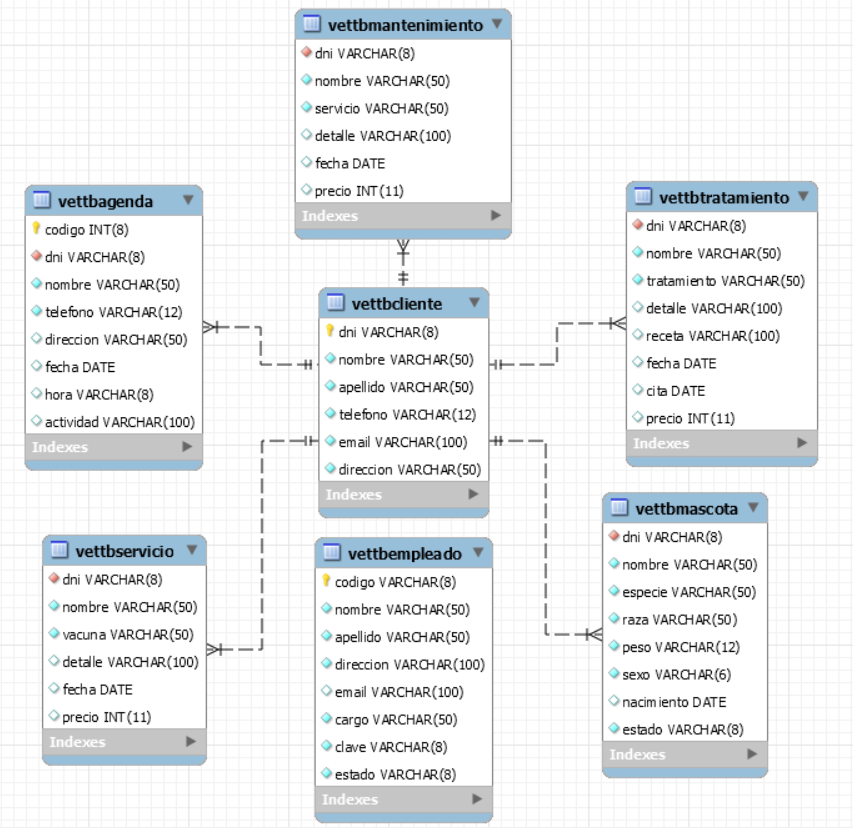
\includegraphics[width=8cm, height=8cm]{img/OR/mapa.png}
							\end{figure}
							
							\begin{figure}[htb]
									\centering 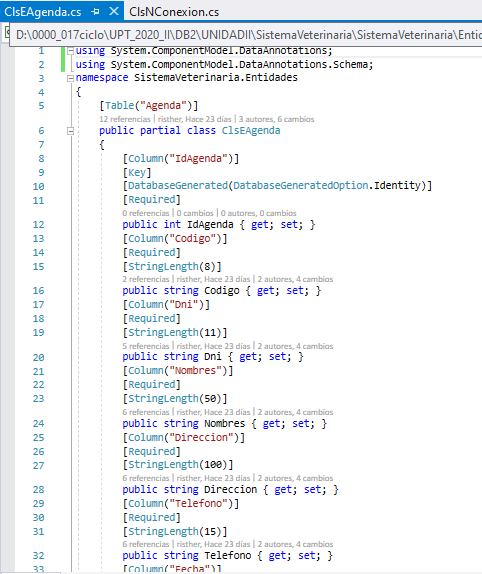
\includegraphics[width=8cm, height=8cm]{img/OR/primera.png}
							\end{figure}
							
							\begin{figure}[htb]
								\centering 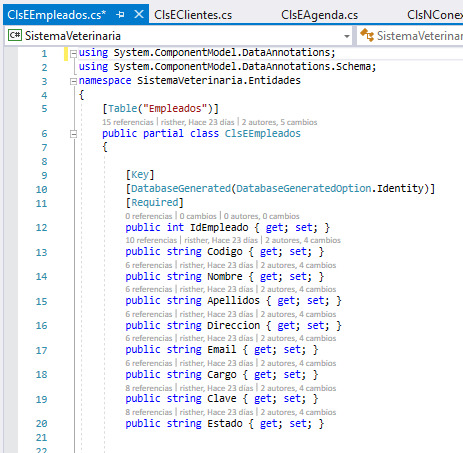
\includegraphics[width=8cm, height=8cm]{img/OR/segunda.png}
							\end{figure}
						
							\begin{figure}[htb]
								\centering 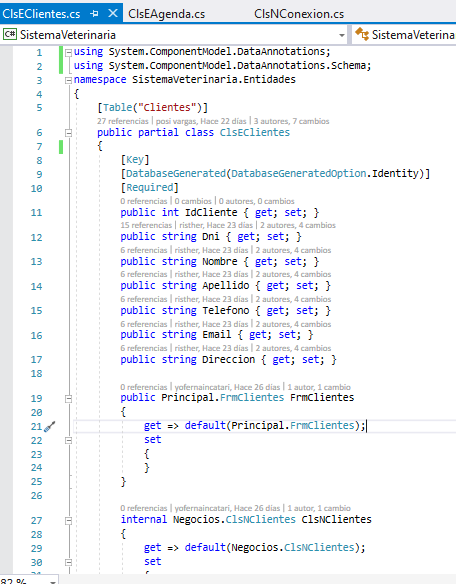
\includegraphics[width=8cm, height=8cm]{img/OR/tercera.png}
							\end{figure}
				\newpage	
						
						
				
					
						\item \textbf{Migraciones.} \\
						
							Nos vamos al Archivo Web.config del proyecto y agregamos lo siguiente.\\
								\begin{figure}[htb]
									\centering 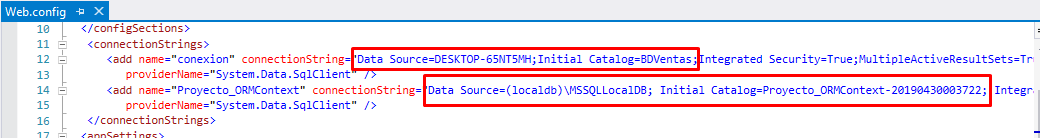
\includegraphics[width=12cm, height=3cm]{img/Migraciones/1webconfig.png}
								\end{figure}
				\newpage			
							La clase Proyeco-ORMContext-cs \\
								\begin{figure}[htb]
									\centering 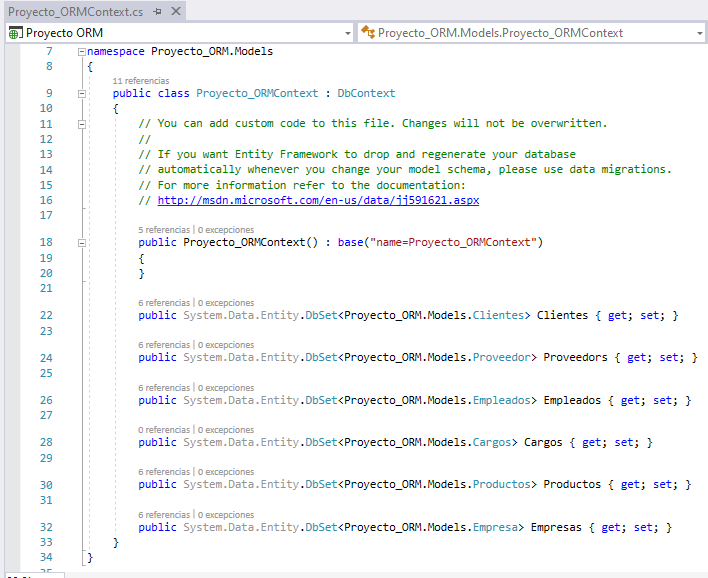
\includegraphics[width=12cm, height=9cm]{img/Migraciones/2Context.png}
								\end{figure}
							
							La carpeta donde est\'an las clases para la migraci\'on \\
								\begin{figure}[htb]
									\centering 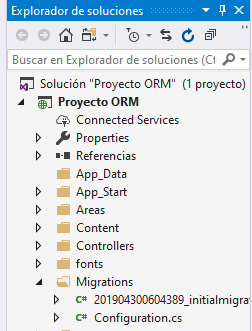
\includegraphics[width=5cm,height=6cm]{img/Migraciones/3clases.png}
								\end{figure}
					
					\newpage
							La clase donde se inicia la migraci\'on 201904300604389-initialmigration-cs  \\
							
								\begin{figure}[htb]
									\centering 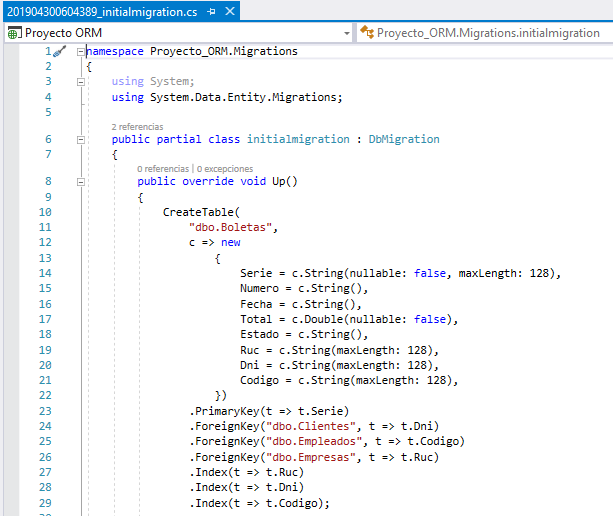
\includegraphics[width=12cm, height=9cm]{img/Migraciones/4clasemigra.png}
								\end{figure}
								
								\begin{figure}[htb]
									\centering 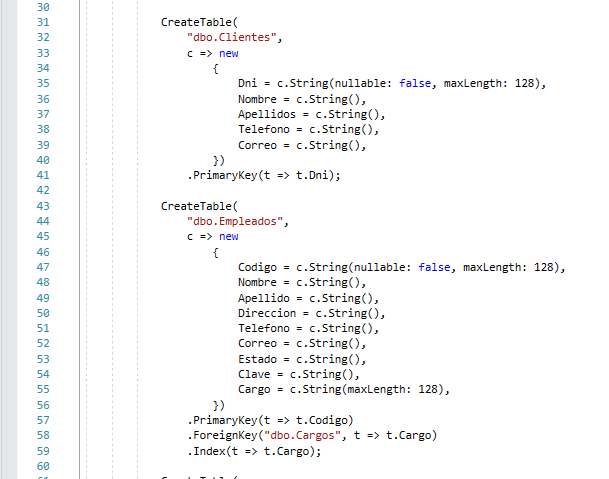
\includegraphics[width=12cm, height=9cm]{img/Migraciones/5clasemigra.png}
								\end{figure}
					\newpage		
								\begin{figure}[htb]
									\centering 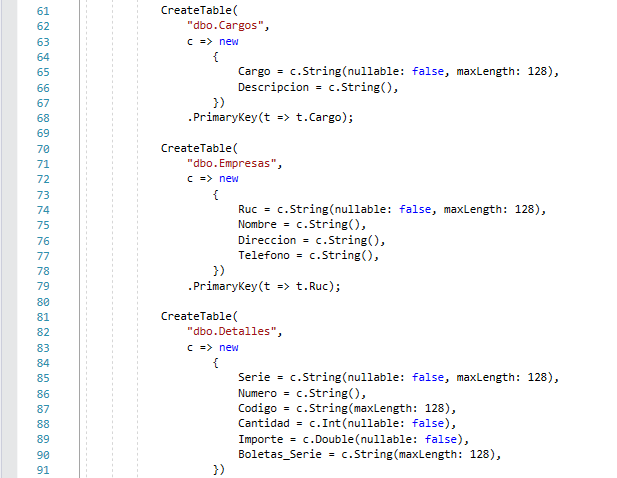
\includegraphics[width=12cm, height=9cm]{img/Migraciones/6clasemigra.png}
								\end{figure}
							
								\begin{figure}[htb]
									\centering 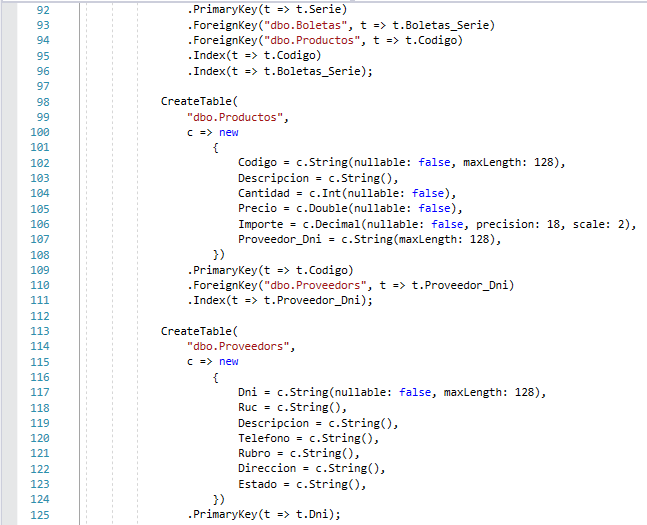
\includegraphics[width=12cm, height=9cm]{img/Migraciones/7clasemigra.png}
								\end{figure}
					\newpage		
								\begin{figure}[htb]
									\centering 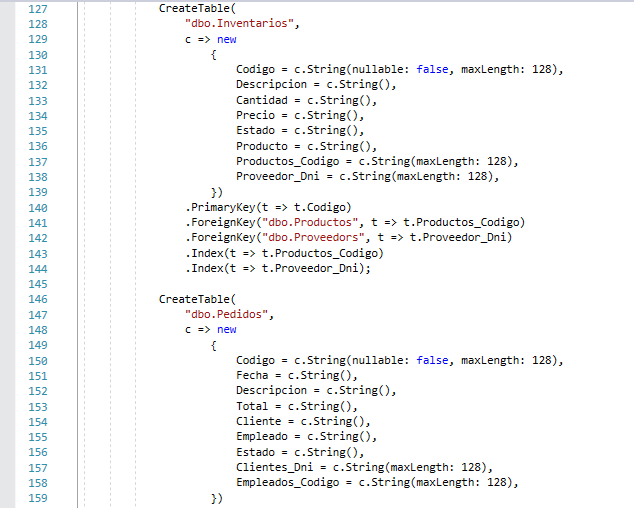
\includegraphics[width=12cm, height=9cm]{img/Migraciones/8clasemigra.png}
								\end{figure}
								
								\begin{figure}[htb]
									\centering 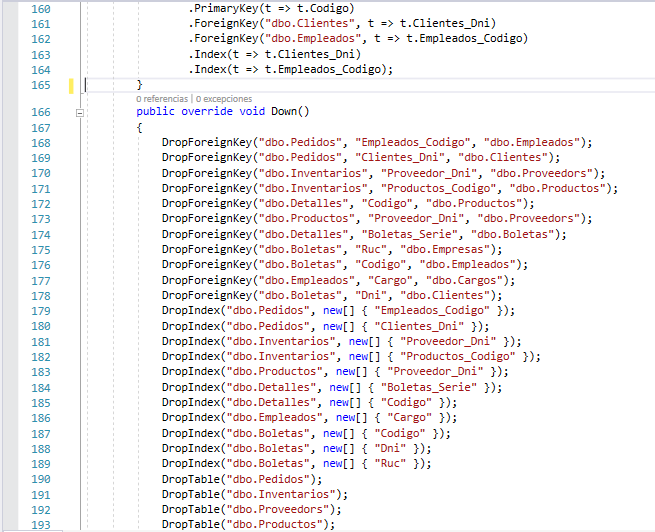
\includegraphics[width=12cm, height=9cm]{img/Migraciones/9clasemigra.png}
								\end{figure}
					\newpage	
								\begin{figure}[htb]
									\centering 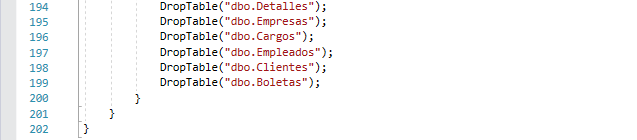
\includegraphics[width=12cm, height=4cm]{img/Migraciones/10clasemigra.png}
								\end{figure}
							
							
							La clase donde se configura la migraci\'on Configuration.cs  \\
								\begin{figure}[htb]
									\centering 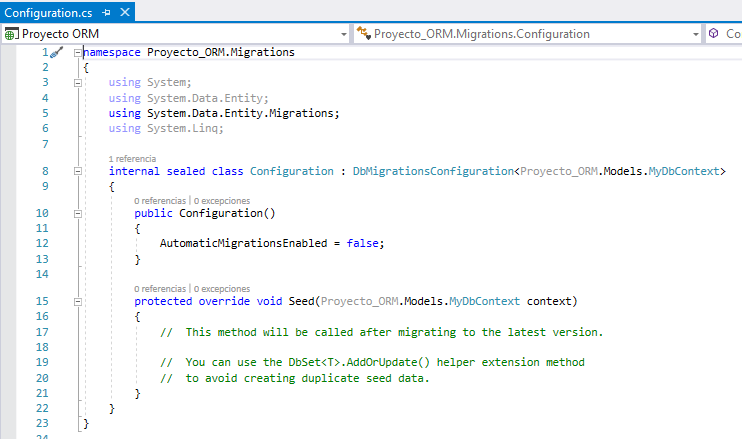
\includegraphics[width=12cm, height=9cm]{img/Migraciones/11configuracion.png}
								\end{figure}
					\newpage
							Comandos para la migraci\'on.\\
								\begin{figure}[htb]
									\centering 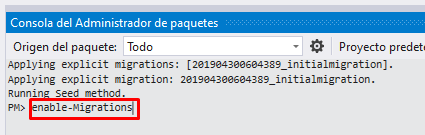
\includegraphics[width=8cm, height=3cm]{img/Migraciones/12comandos.png}
								\end{figure}
							
								\begin{figure}[htb]
									\centering 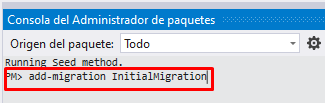
\includegraphics[width=8cm, height=3cm]{img/Migraciones/13comandos.png}
								\end{figure}
							Se ve que el servidor no tiene la base de datos DBVentas.  \\
								\begin{figure}[htb]
									\centering 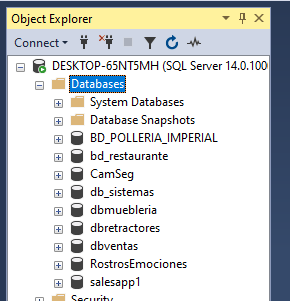
\includegraphics[width=8cm, height=10cm]{img/Migraciones/14datos.png}
								\end{figure}
					\newpage			
							Con este comando logramos que migre y cree la base de datos del proyecto  \\
								\begin{figure}[htb]
									\centering 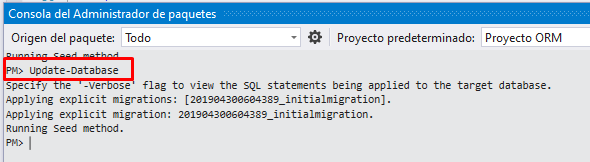
\includegraphics[width=8cm, height=3cm]{img/Migraciones/15consola.png}
								\end{figure}
							Como se puede ver se crea la base de datos de nuestro proyecto  \\
								\begin{figure}[htb]
									\centering 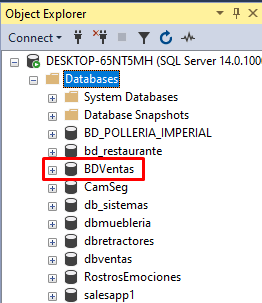
\includegraphics[width=8cm, height=10cm]{img/Migraciones/16view.png}
								\end{figure}
					\newpage		
							Dentro de la base de datos estan todas las propiedades de nuestras clases del proyecto asi como las clases mismas.  \\
								\begin{figure}[htb]
									\centering 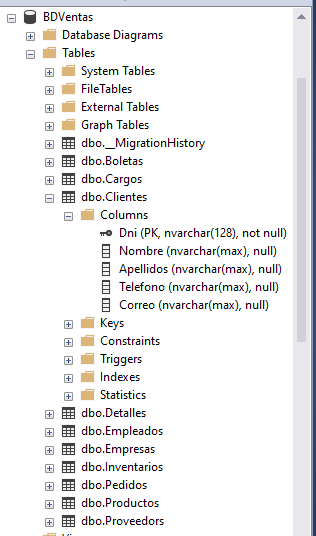
\includegraphics[width=5cm, height=8cm]{img/Migraciones/17complet.png}
								\end{figure}
			\newpage
						
					
								\begin{table}[t]
									
								\item \textbf{Diccionario de datos.} \\
						  	
									\begin{tabular}{| c | c | c | c | }
										\hline
										\multicolumn{4}{ |c| }{\textbf{Formulario FrmClientes}} \\ \hline
										\textbf{Campo} & \textbf{Tamaño} & \textbf{Tipo de Dato} & \textbf{Descripción} \\  
										
										\hline
										txtDni	& 8 & varchar & DNI del cliente. \\
										txtNombre & 50 & varchar & Nombres del cliente. \\
										txtApellido & 50 & varchar & Apellido Paterno y Materno del cliente. \\
										txtTelefono & 12 & varchar & Número telefónico del cliente. \\
										txtEmail & 100 & varchar & Email del cliente. \\
										txtDireccion & 50 & varchar & Dirección familiar del cliente. \\
										txtBuscar & 8 & varchar & Búsqueda del cliente a través del DNI. \\
										dgvCliente & - & general & Muestra todo el registro del FrmClientes. \\  
										
										\hline
										
									\end{tabular}
									\label{tab:coches}
								\end{table}
						
								\begin{table}[t]
								\begin{tabular}{| c | c | c | c | }
									\hline
									\multicolumn{4}{ |c| }{\textbf{Formulario FrmEmpleados}} \\ \hline
									\textbf{Campo} & \textbf{Tamaño} & \textbf{Tipo de Dato} & \textbf{Descripción} \\  
									
									\hline
										txtCodigo & 8 & varchar & Código del empleado. \\ 
										txtNombre & 50 & varchar & Nombres del empleado. \\ 
										txtApellido & 50 & varchar & Apellido Paterno y Materno del empleado.\\ 
										txtDireccion & 50 & varchar & Dirección familiar del empleado.\\ 
										txtEmail & 100 & varchar & Email del empleado.\\ 
										cbCargo	& 50 & varchar & Cargo del empleado.\\ 
										txtClave & 8 & varchar & Clave asignado al empleado.\\ 
										rbEstado & 8 & varchar & Estado actual del empleado.\\ 
										txtBuscar & 8 & varchar & Búsqueda al empleado por su código.\\ 
										dgvEmpleado & -	& general & Muestra todo el registro del FrmEmpleados.\\   
									
									\hline
									
								\end{tabular}
								\label{tab:FrmEmpleados}	
							\end{table}
						
								
								
								\begin{table}[t]
								\begin{tabular}{| c | c | c | c | }
									\hline
									\multicolumn{4}{ |c| }{\textbf{Formulario FrmMascotas}} \\ \hline
									\textbf{Campo} & \textbf{Tamaño} & \textbf{Tipo de Dato} & \textbf{Descripción} \\ 
									
									\hline
									txtDni	& 8 & varchar & Documento Nacional de Identidad del cliente.\\
									txtNombre & 50	& varchar & Nombre de la mascota del cliente.\\
									txtEspecie & 50	& varchar & Especie de la mascota del cliente.\\
									txtRaza	& 50 & varchar	& Raza de la mascota del cliente.\\
									txtPeso	& 12 & varchar	& Peso de la mascota del cliente.\\
									txtSexo & 6 & varchar	& Género de la mascota del cliente.\\
									txtNacimiento & - & date & Fecha del nacimiento de la mascota.\\
									txtEstado & 8 & varchar & Estado actual de la mascota del cliente.\\
									txtBuscar & 8 & varchar & Búsqueda de la mascota por el DNI.\\
									dgvCliente & max & general & Muestra todo el registro del FrmMascotas.\\  
									
									\hline
									
								\end{tabular}
							
								\label{tab:FrmMascotas}
							\end{table}
				
								
								
								\begin{table}[t]
								\begin{tabular}{| c | c | c | c | }
									\hline
									\multicolumn{4}{ |c| }{\textbf{Formulario FrmServicioVacunación}} \\ \hline
									\textbf{Campo} & \textbf{Tamaño} & \textbf{Tipo de Dato} & \textbf{Descripción} \\  
									
									\hline
										txtDni	& 8 & varchar & Documento Nacional de Identidad del cliente.\\ 
										txtNombre & 50 & varchar & Nombre de la mascota del cliente.\\ 
										txtVacuna & 50 & varchar & Tipo de vacuna del servicio clínico.\\ 
										txtDetalle & 100 & varchar & Detalle de la aplicación de la vacuna.\\ 
										txtFecha & - &	date & Fecha de la aplicación de la vacuna.\\ 
										txtPrecio & 11 & int &	Precio de la aplicación de la vacuna.\\ 
										txtBuscar & 8 &	varchar & Búsqueda de la vacuna por el DNI de cliente.\\ 
										dgvVacunas & max & General & Muestra todo el registro del FrmServicios.\\    
									
									\hline
									
								\end{tabular}
								\label{tab:FrmServicioVacunación}
						\end{table}
					
								
								
								\begin{table}[t]
								\begin{tabular}{| c | c | c | c | }
									\hline
									\multicolumn{4}{ |c| }{\textbf{Formulario FrmMantenimientoMascota}} \\ \hline
									\textbf{Campo} & \textbf{Tamaño} & \textbf{Tipo de Dato} & \textbf{Descripción} \\  
									
									\hline
									txtDni & 8 & varchar & Documento Nacional de Identidad. \\
									txtNombre & 50 & varchar & Nombre de la mascota del cliente. \\
									txtServicio & 50 & varchar & Tipo de servicio clínico. \\
									txtDetalle & 100 & varchar & Detalle del servicio clínico ofrecido. \\
									txtFecha & - & date & Fecha del servicio ofrecido. \\
									txtPrecio & 11 & int & Precio del servicio ofrecido. \\
									txtBuscar & 8 & varchar & Búsqueda del servicio por el DNI de cliente. \\
									dgvMantenimiento & max & general & Muestra todo el registro del Formulario. \\   
									
									\hline
									
								\end{tabular}
								\label{tab:FrmMantenimientoMascota}
							\end{table}
							
								
						
								\begin{table}[t]
									
								\begin{tabular}{| c | c | c | c | }
									\hline
									\multicolumn{4}{ |c| }{\textbf{Formulario FrmTratamientoMascota}} \\ \hline
									\textbf{Campo} & \textbf{Tamaño} & \textbf{Tipo de Dato} & \textbf{Descripción} \\  
									
									\hline
									txtDni & 8  & varchar  & Documento Nacional de Identidad del cliente. \\ 
									txtNombre & 50  & varchar  & Nombre de la mascota del cliente. \\ 
									txtTratamiento &  50 & varchar & Tipo de tratamiento clínico ofrecido. \\ 
									txtDetalle & 100 & varchar  & Detalle del tratamiento clínico ofrecido.\\ 
									txtReceta & 100 & varchar  & Receta del tratamiento clínico ofrecido. \\ 
									txtFecha & -  & date  &	Fecha del tratamiento ofrecido. \\ 
									txtCita & -  & date  &	Fecha de la próxima cita del tratamiento. \\ 
									txtPrecio & 11  & int   &Precio del servicio ofrecido. \\ 
									txtBuscar & 8  & varchar  & Búsqueda del servicio por el DNI de cliente. \\ 
									dgvTratamiento & max  &	general & Muestra todo el registro del FrmTratamiento. \\   
									
									\hline
									
								\end{tabular}
								\label{tab:FrmTratamientoMascota}
							\end{table}
								
								\begin{table}[t]
									
								\begin{tabular}{| c | c | c | c | }
									\hline
									\multicolumn{4}{ |c| }{\textbf{Formulario FrmAgenda}} \\ \hline
									\textbf{Campo} & \textbf{Tamaño} & \textbf{Tipo de Dato} & \textbf{Descripción} \\ 
									
									\hline
									txtDni & 8 &varchar & Documento Nacional de Identidad del cliente. \\
									txtNombre & 50 & varchar & Nombres del cliente. \\
									txtApellido & 50 & varchar & Apellido Paterno y Materno del cliente. \\
									txtTelefono & 12 & varchar & Número telefónico del cliente. \\
									txtFecha & - &	date & Fecha del próximo evento programado. \\
									txtHora	& 6 & varchar & Hora del evento programado. \\
									txtActividad & 100 & varchar & Descripción de la actividad programada. \\
									txtBuscar & - &	date & Búsqueda por fecha de la agenda. \\
									dgvAgenda & max & general & Muestra el registro del formulario agenda. \\ 
									
									\hline
									
								\end{tabular}
								\label{tab:FrmAgenda}	
									
								\end{table}
						
							
				

					\end{enumerate}
				
				
				
				
			\end{enumerate}
			
		  
	\end{enumerate}
	
	

\end{document}
